\documentclass[10pt,letterpaper]{article}
\usepackage[margin=0.93in,top=0.86in,bottom=0.85in]{geometry}
\usepackage[T1]{fontenc}
\usepackage{lmodern,amsmath,amssymb,amsthm,booktabs,graphicx,xcolor,microtype}
\usepackage{enumitem,fancyhdr,hyperref}
\definecolor{pine}{HTML}{234C43}
\definecolor{slate}{HTML}{526661}
\hypersetup{colorlinks=true,linkcolor=pine,urlcolor=pine,citecolor=pine,
 pdftitle={Intrinsic diameter and farthest points of a parallelepiped},pdfauthor={OpenAI}}
\newtheorem{theorem}{Theorem}
\setlist{nosep,topsep=4pt,leftmargin=1.65em}
\setlength{\parskip}{2.2pt}
\setlength{\emergencystretch}{2em}
\pagestyle{fancy}\fancyhf{}
\fancyhead[L]{\small\sffamily\color{slate}Farthest points on a parallelepiped}
\fancyhead[R]{\small\sffamily\color{slate}Intrinsic geometry}
\fancyfoot[C]{\small\sffamily\thepage}
\renewcommand{\headrulewidth}{0.25pt}
\setlength{\headheight}{14pt}
\begin{document}
\thispagestyle{plain}
\begin{center}
{\large\sffamily\color{pine}Polyhedral surface geometry}\\[7pt]
{\LARGE\bfseries Intrinsic diameter and farthest points\\[3pt]
of a parallelepiped}\\[7pt]
{\normalsize Exact coordinates from face developments and a proof in finite arithmetic}\\[6pt]
{\small Prepared for Vladimir Reshetnikov \(\cdot\) November 19, 2026}
\end{center}
\noindent
A prescribed vertex can have its unique farthest point inside a face.
With both endpoints free, every diametral pair is centrally opposite,
but its endpoints can both lie inside faces. We give finite formulas
for the coordinates and attained lengths for every nondegenerate
parallelepiped. The fixed-vertex formula uses only field operations,
square roots and comparisons. The unrestricted formula adds real
roots of degree at most four over the developed face data. A rational
example attains degree four for the squared diameter.

\section{The input and the two answers}\label{sec:start}
Let $e_1,e_2,e_3$ issue from one vertex $o$ and have positive lengths
$l_i$. Specify their pairwise angles $\theta_{ij}$ through
\[
 G_{ii}=l_i^2,\qquad G_{ij}=l_i l_j\cos\theta_{ij},\qquad
 X(u)=o+\sum_{i=1}^3u_i e_i,\qquad u\in[0,1]^3 .
\]
The symmetric matrix $G$ must be positive definite. Its first three
leading principal minors being positive is an equivalent test. Angles
determine shape only after the three lengths (up to a common scale
for scale-free answers) are also supplied. The boundary
$S$ consists of the six closed faces $F_{i,b}=\{u_i=b\}$,
$b=0,1$. The intrinsic distance $d(p,q)$ uses only paths in $S$,
with length measured in ordinary Euclidean space after applying $X$.
The prescribed vertex $v$ is given by its three bits. Put
\[
 E(v)=\max_{q\in S}d(v,q),\qquad D=\max_{p,q\in S}d(p,q),\qquad
       Iu=(1-u_1,1-u_2,1-u_3).
\]
For named real data a maximum value in these formulas is interpreted
by the certified suprema of Section~\ref{sec:names}. Returned points
are in edge coordinates, giving Cartesian coordinates immediately
by $X$. If only lengths and angles are available, take the columns
\[
 e_1=(l_1,0,0),\quad e_2=(G_{12}/l_1,b,0),\quad b=\sqrt{G_{22}-G_{12}^2/G_{11}},
\]
\[
 e_3=\left(G_{13}/l_1,\frac{G_{23}-G_{12}G_{13}/G_{11}}b,
                   \frac{\sqrt{\det G}}{l_1 b}\right).
\]
Their Gram products give $G$. A different rigid placement transports
the answer. If the input angles are \emph{interior dihedral angles}
$\delta_{ij}$ between the two incident faces opposite axes $i,j$ in
the trihedral angle at $o$ (the faces $u_i=0,u_j=0$), first form
the Gram matrix $N$ of their inward unit normals, $N_{ii}=1$,
$N_{ij}=-\cos\delta_{ij}$. Their dual basis points along the three
positive edges, with Gram matrix $N^{-1}$. Consequently
$\cos\theta_{ij}=(N^{-1})_{ij}/\sqrt{(N^{-1})_{ii}(N^{-1})_{jj}}$.

\paragraph{How to get coordinates and the length.}
For the fixed vertex use the corners, edge--bisector intersections
and circumcenters of Section~\ref{sec:fixed-images}. For free endpoints
use the corners, edge roots and triple equalities of
Section~\ref{sec:quartic} on the three faces $u_i=0$. In either
list take the shortest \emph{admissible} developed length at each
point, then take the largest of these scores. A winning first-list
point $q$ returns $(v,q,E(v))$. A winning second-list point $p$
returns $(p,Ip,D)$. Freeing the endpoints helps precisely when the
winning second-list length exceeds $d(v,Iv)$, by \eqref{eq:gap}.
These rules include ties and right angles without perturbing the input.

\begin{figure}[htb]
\centering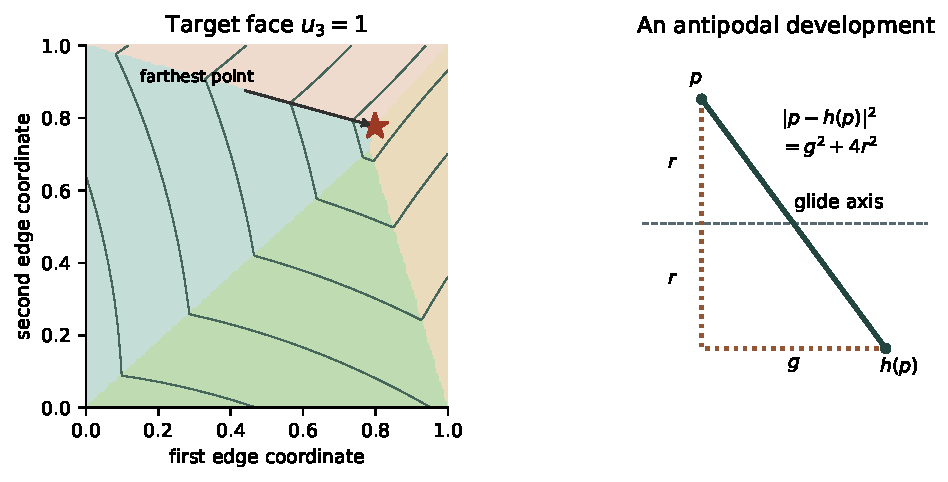
\includegraphics[width=.91\linewidth]{surface_geometry.pdf}
\caption{In the left panel the colors mark winning developments to the top
face of the skew $1,1,2$ example in Section~\ref{sec:worked-quartic}.
Contours show intrinsic distance from the origin. The marked point
has exact coordinates $(1281/1604,1247/1604,1)$. In the right panel unfolding a
centrally reflected endpoint gives a glide reflection. The perpendicular
part of the displacement is twice the signed distance to its axis.}
\end{figure}
\paragraph{Relation to the supplied archives.}
The two supplied reports give side-length regimes for cuboids.
A general affine deformation preserves face incidences and changes
each face metric. The present calculation uses the Gram form on every
chord, derives its candidate lists afresh and recovers, for example,
the fixed result $E^2=65/8$ at edge coordinates $(3/4,3/4,1)$ in
the rectangular $1,1,2$ case. Nikonorov and Nikonorova's published
formula concerns rectangular parallelepipeds \cite{rect}. The
antipodal comparison extends beyond boxes \cite{nik}.

\section{From continuous surface curves to six face chords}
\label{sec:finite-metric}

Write $u=(u_1,u_2,u_3)\in[0,1]^3$ for affine cube coordinates.
Let $T u=\sum_i u_i e_i$, where $e_1,e_2,e_3$ are the independent edge
vectors at a chosen reference vertex. A common physical translation is
immaterial. The Gram matrix is $G=(e_i\mathbin{\cdot}e_j)$. Put
$H=\sum_i |e_i|$ and $K=\max_i|e_i|$. Two points of a face have chord
length
\[
  c(u,v)=\sqrt{(u-v)^{\mathsf T}G(u-v)},\qquad
  c(u,v)\le H\|u-v\|_\infty .
\]
Denote the face $u_i=b$ by $(i,b)$, for $b\in\{0,1\}$. Distinct faces
share a closed edge exactly when their indices $i$ differ. At a boundary
point one may use any incident face as its chart.

Fix endpoint charts $f$ and $g$ containing $x$ and $y$, respectively.
A word $w=(f_0,\ldots,f_k)$ starts at $f$, ends at $g$, has pairwise
distinct faces, and each consecutive pair shares an edge. For the $j$th
shared edge, $1\le j\le k$, write $z_j(t_j)$ for the point obtained by
fixing the two named coordinates and setting the remaining coordinate
equal to $t_j\in[0,1]$. With $z_0=x$, $z_{k+1}=y$, put
\begin{equation}
  L_w(x,y;t)=\sum_{j=0}^k c(z_j,z_{j+1}).
  \label{eq:metric-chain}
\end{equation}
Each segment belongs to the specified closed face by its convexity.
There are at most five edge parameters. For prescribed charts the word
counts are one when $f=g$, 26 for adjacent charts and 28 for opposite
charts. They can be verified by starting a word with $f$ and appending
each unused face of a different index from the current last face,
recording a word whenever its last face is $g$.

\paragraph{A constructive metric theorem.}
The infimum of \eqref{eq:metric-chain} over these words and their edge
parameters is the intrinsic distance for continuous surface paths.
Here the lower-bound assertion for a curve has a finite meaning. For
each error $\varepsilon>0$ there is a finite, ordered set of its
sample times for which the sum of sample chords, plus $\varepsilon$,
bounds the infimum from above. Thus every upper bound on the curve's
length bounds the distance. The reverse comparison uses the polygonal
paths from \eqref{eq:metric-chain}. This formulation also applies when
one has no real-valued total-variation functional for an input curve.

\paragraph{Proof.}
Represent a continuous curve in cube coordinates by a uniformly
continuous name with a supplied modulus $\omega$. For example,
$|s-t|\le2^{-\omega(n)}$ guarantees
$\|u(s)-u(t)\|_\infty\le2^{-n}$. Fix $h=2^{-n}<1/8$, and sample at
the $N+1$ times $i/N$, where $N=2^{\omega(n)}$. Score each of the six
boundary planes at a sample by its coordinate distance, using rational
coordinate approximations with error at most $h/4$. Choose the least
index achieving the smallest rational score. The true distance from the
sample to its chosen plane is at most $h/2$, since the true minimum is
zero and scores change by at most $h/4$. At the initial and terminal
times use the given charts instead. Opposite faces cannot label two
consecutive samples, since their unit separation would be at most
$h/2+h+h/2<1$.

Start at sample index $s=0$. Keep its label and find the last index
$i\ge s$ with that label. If $i=N$ the word is finished. Otherwise
record a transition at $i/N$, set $s=i+1$, and repeat. An earlier kept
label never recurs after its own last occurrence. There are at most
six kept labels. The consecutive retained labels at a transition were
the original labels of consecutive samples $i$ and $i+1$. They are
distinct and cannot be opposite, hence define a shared edge. At time
$i/N$, the coordinate distance from the sample to the first plane
is at most $h/2$, and to the second at most $h+h/2$. Snap its two
specified coordinates to these planes, leaving the third coordinate in
$[0,1]$. The physical displacement is at most $2Hh$. One may use a
rational approximation to the third coordinate of error $h/4$,
clipped to $[0,1]$, with the same bound. Connect these snapped points,
in order, between $x$ and $y$. They give exactly the type of path in
\eqref{eq:metric-chain}. Each of the at most five snapped points
contributes at most twice its displacement to the chord sum, by the
triangle inequality. Its length therefore exceeds the chord sum at
the selected sample times by at most $20Hh$. Repeated endpoint times
are harmless, as their chord lengths vanish. Taking arbitrarily small
$h$ proves the lower-bound assertion. Conversely, every word and every
parameter tuple gives a continuous surface path of the stated length by
linear interpolation in its successive faces. This proves the claim
and proves independence of endpoint chart choices.

\paragraph{Uniform rational evaluation.}
If $t_j$ is replaced by a multiple of $1/M$ within $1/M$, its physical
displacement is at most $K/M$. The two adjacent summands change by at
most $2K/M$. Thus restricting all crossings to the edge grid raises the
infimum by at most $10K/M$. This statement can be used for real names
without comparing them to grid boundaries by first approximating a parameter
to within $1/(4M)$, rounding the approximation to the nearest grid point,
and clipping. The total error in that parameter is at most $3/(4M)$.
Let $d_M$ be the minimum of the finitely many resulting lengths. Then
\[
     d_M-10K/M\ \le\ d(x,y)\ \le\ d_M .
\]
The proof of these inequalities constructs the distance as a Cauchy
value. For instance nested dyadic grids have $d_{2M}\le d_M$ and
$d_M-d_{2^jM}\le10K/M$ for every $j$. Approximating each grid length
to $\eta$ approximates the finite minimum to $\eta$ and choosing a
least approximate length gives a path within $2\eta+10K/M$ of optimal.
Finite minima of Cauchy values here are value operations
$\min(a,b)=(a+b-|a-b|)/2$. Selecting a minimizing index only uses
rational comparisons of approximations. Given an integer upper bound
for $H$, the mesh for a requested binary precision can be chosen by
multiplication by a power of two. Sample counts, word bounds, grid
sizes and the precision of square roots (by bounded bisection) are
therefore primitive recursive. The curve-specific bound is primitive
recursive relative to its supplied modulus. For a fixed primitive
recursive modulus it is an ordinary primitive recursive bound.

\section{When straight planar developments can be used}
\label{sec:legal-nets}

For algebraic input coordinates and positive definite algebraic $G$,
each product of closed shared edges is a closed bounded algebraic box.
The length sum in \eqref{eq:metric-chain} is continuous and
semialgebraic. Introduce a nonnegative length variable for each term
and impose its squared chord equation. Each word has a minimum with
real algebraic coordinates, by closed bounded semialgebraic
optimization (equivalently by real closed field elimination and
algebraic sample selection). A minimum across the finite word list
is therefore an actual intrinsic shortest path. This use of algebraic
optimization is at fixed dimension and fixed algebraic format in the
Gram entries and endpoint coordinates. Integer elimination bounds,
and an alternative grid formulation for Cauchy names, are discussed
elsewhere in this report.

A shortest nonconstant path has no vertex in its interior. To see the
strict cone-angle inequality at a vertex, take the three unit outward
edge directions $a,b,c$ there, putting
$\alpha=\angle(a,b)$, $\beta=\angle(b,c)$ and
$\gamma=\angle(a,c)$. The perpendicular projections of $a$ and $c$
onto $b^\perp$ are nonzero and noncollinear by independence. Their dot
product is strictly greater than the negative product of their lengths.
Consequently
\[
  \cos\gamma>\cos\alpha\cos\beta-\sin\alpha\sin\beta.
\]
If $\alpha+\beta\le\pi$, then
$\alpha+\beta+\gamma<2\pi$ because $\gamma<\pi$.
Otherwise comparison of cosines gives
$\gamma<2\pi-\alpha-\beta$. In both cases the sum of the three face
angles, i.e. the cone angle, is strictly below $2\pi$. At a purported
interior vertex of our polygonal minimizer take sufficiently short
initial pieces of the rays leading to its predecessor and successor.
One of the two surface sectors between the rays has total angle
strictly below $\pi$. Developing that sector gives a convex planar
sector. The chord between the two small ray endpoints stays in this
sector and is strictly shorter than the broken path through its
apex. The radius can be chosen below the distance to every
nonincident edge, so this local substitution is a surface path.
Equal rays give an immediate shortening by deletion. This contradicts
minimality. The angle vocabulary abbreviates algebraic predicates. Orientations and dot products of planar rays compare angles up to
$\pi$, and $\sin\alpha,\sin\beta$ are positive square roots of
$1-\cos^2\alpha,1-\cos^2\beta$. Angles need not be computed by an
inverse trigonometric operation.

Across an interior point of an edge, lay the two incident faces on
opposite sides of their common line. In a sufficiently small disk the
surface is now flat. A bend would admit a strictly shorter chord inside
the disk. The same argument applies inside each face. Hence a shortest
polygonal path develops to one straight segment in a simple face word.
A positive-length portion running along an edge continues along the
same line until an endpoint, since departure would cause a bend and an
interior vertex has just been excluded. Endpoint charts can add a
zero-length initial or terminal segment. Interior zero-length face
pieces between two distinct seams would require a vertex and can be
discarded in a constant path.

For an explicit development, embed the first face isometrically in the
plane with its first generating edge horizontal, and deploy each next
face across its actual shared segment $AB$. With
$E=(B-A)/|B-A|$ and $J$ counterclockwise rotation through $\pi/2$,
an adjacent edge vector $v$ from $A$ has planar image
\[
   sE\ \mathbin{\pm}\sqrt{|v|^2-s^2}\,JE,\qquad
   s=\frac{v\cdot (B-A)_{\mathrm{sp}}}{|B-A|}.
\]
Here $(B-A)_{\mathrm{sp}}$ is the corresponding oriented spatial edge
vector, and the sign puts the next face in the half-plane opposite
the preceding face. The remaining corner follows by parallelogram
addition. All operations use the input Gram matrix and positive square
roots. With developed endpoint images $P,Q$, test whether the segment
$P+\lambda(Q-P)$ intersects each successive closed seam at parameters
$0\le\lambda_1\le\cdots\le\lambda_k\le1$ in the required order.
Equivalently solve
\[
   P+\lambda_j(Q-P)=A_j+t_j(B_j-A_j),\qquad 0\le t_j\le1
\]
for all seams with these order bounds. This system handles collinear
seams, zero steps and vertex hits. Face convexity puts each segment
between consecutive seam points in the prescribed face, so the test is
both necessary and sufficient for this particular straight development.
Developments may overlap elsewhere in the plane without affecting
the test. Every accepted segment has length $|Q-P|$ and is realizable.
At least one accepted segment realizes the minimum by the preceding
argument. Thus the minimum over accepted developments equals the
distance. The infimum formula \eqref{eq:metric-chain} and its uniform
error estimate do not require decidable segment incidence on arbitrary
real names.

\paragraph{The graph used by the accompanying calculator.}
For rational $G$, subdivide every edge into $m$ equal parts, identify
common corners, and join every pair of nodes sharing a face. Insert
query endpoints with the same adjacency rule and include their direct
chord when they share a face. The graph has $12m-4$ boundary nodes
before query insertion. Assign a chord of squared length $s$ the
integer cost $\lceil W\sqrt{s}\rceil$. A shortest graph route of cost
$C$ gives an actual surface path of length at most $C/W$. Conversely,
on an optimal simple face route, rounding each crossing to the nearest
edge node displaces it by at most $K/(2m)$. The resulting path has at
most six chords, so
\[
       C/W-5K/m-6/W\ \le\ d(x,y)\ \le\ C/W .
\]
For algebraic input, nearest-node ties are decidable. The calculator
uses rational input and forms all squared lengths as integers divided
by a common denominator, using integer square roots to certify every
rounding. Its $K$ is a rational upper bound on the longest edge.
The ambient chord is also a lower bound. On an $n$-subdivision grid
in each face a point can be moved to its nearest coordinate grid point
with surface displacement at most $(|e_i|+|e_j|)/(2n)\le K/n$.
Hence the fixed-vertex maximum is enclosed by the maximum sampled
lower bound and the maximum sampled upper bound plus $K/n$.
For a pair related by central reflection the same move changes the
distance by at most $2K/n$, giving the corresponding antipodal
maximum enclosure. A coordinate pair realizing the largest sampled
lower bound is an explicit approximate witness.

\section{Ten images and a finite formula for a selected vertex}
\label{sec:fixed-images}

Choose the selected vertex as affine origin and use its three outgoing
edges as generators. If its old binary coordinates were $v_i$, the new
vectors are $(1-2v_i)e_i$ and the new coordinates are
$(1-2v_i)(u_i-v_i)$. This describes the same solid and accounts for
the requisite sign changes in the Gram matrix. Call the three incident
faces negative and the other three positive.

On a negative face the straight chord from the origin is available, so
a farthest point on that face occurs among its four corners. On a
positive target face $F$, choose a Cartesian development of $F$ itself.
Begin a word with one negative face and continue through distinct
positive faces, ending at $F$, with consecutive faces adjacent. Develop
backwards from $F$ and record the planar source image $s_j$ and the seams.
To see completeness, take a shortest polygonal path and consider the
last negative face in its word. Replace its entire prefix up to its
last contact on that face by the chord in the face from the source.
A shorter prefix would contradict minimality. The resulting shortest
path has the required word, allowing contacts at endpoints. For a
target opposite negative face 3 the positive suffixes from negative
face 1 are $3$, $2,3$, $2,1,3$. From negative face 2 interchange 1
and 2 in that list. From negative face 3 the suffixes are $1,3$,
$2,3$, $1,2,3$, $2,1,3$. Thus there are ten words. Distinct words
with the same planar source image retain their own legality tests.

\paragraph{Coordinates of a farthest point.}
In the target face draw the Euclidean bisectors of its distinct sites
$s_j$. Form the following finite set $V_F$, retaining points of the
closed parallelogram.
\begin{enumerate}
\item The four corners.
\item Every intersection of an edge with a nonparallel site bisector.
\item The circumcenter of every noncollinear triple of sites.
\end{enumerate}
For a negative face use only its corners. On a positive face, for each
$q\in V_F$ put
\[
 b_F(q)=\min\{\,|q-s_j|^2:\text{word $j$ passes the ordered-seam test at $q$}\,\}.
\]
On negative faces use the squared spatial chord. The fixed-vertex answer
is $\sqrt{\max_F\max_{q\in V_F} b_F(q)}$. Use a winning $q$ and invert
the two generating vectors of its planar face chart to get its affine
coordinates. The bisector equation is
$2(s_j-s_i)\cdot q=|s_j|^2-|s_i|^2$. A circumcenter solves two such
nonsingular linear equations. A winning point and its squared distance
therefore lie in the field obtained from the Gram entries by the square
roots and field operations of the developments. Each positive face
contributes at most $4+4\binom{10}{2}+\binom{10}{3}=304$ candidates.

\paragraph{Why switches of legal words cause no missing maximum.}
Write $b(q)=d(0,q)^2$. The triangle inequality gives
$|d(0,q)-d(0,q')|\le |q-q'|$ on the same face. At every point, $b$
equals at least one $f_j(q)=|q-s_j|^2$. At a particular $q$ call a
site active if $f_j(q)=b(q)$, including every site with that value. In
a neighborhood $b$ always equals a function active at $q$, since the finite
list of other values is separated from $b(q)$, and $b$ and the $f_j$
are continuous. For algebraic data and algebraic $q$ the smallest
positive separation and the face Lipschitz bounds give an explicit
positive radius.

At an interior maximum with a single active site, moving a short
distance in opposite directions makes at least one function value
larger by strict convexity. With exactly two active sites take the
two steps along their bisector. The functions agree and are strictly
convex there. Three distinct sites equidistant from $q$ cannot be
collinear, since a line meets their common circle in at most two
points. This gives item 3. Inside an edge, if all active restrictions
are identical, use strict convexity along the edge. Otherwise two
different restrictions agree at $q$, so their bisector crosses the
edge transversely, giving item 2. Algebraic attainment, used here and
for word lengths, follows from the lemma below.


\section{Why the second endpoint can be the central reflection}
\label{sec:central}
Write $Iu=\mathbf 1-u$. For every two boundary points,
\begin{equation}
   2d(p,q)\ \le\ d(p,Ip)+d(q,Iq).
   \label{eq:cross}
\end{equation}
This is the two-path argument behind Nikonorov's diameter theorem
\cite{nik}. We give a finite polyhedral proof of the needed intersection.
In particular one need not assume a fixed-point theorem for continuous maps.

\paragraph{Intersection lemma.}
Let $A$ be a boundary polygonal path from $p$ to $Ip$, and $B$ one
from $q$ to $Iq$. For algebraic path data, $B$ meets $A\cup I(A)$, and
an intersection point can be found by a bounded calculation.
Do all incidence calculations in the coefficient cube. Subdivide its
faces so that $A,I(A),B,I(B)$ are unions of edges and $I$ acts on the
subdivision. One explicit construction cuts each face by the supporting
lines of the listed segments, marks all segment endpoints, and takes
the union of the subdivisions on a shared cube edge. Include a line
through any isolated marked point in a face, and its reflected line
on the opposite face. Markings on a line subdivide it. Triangulate
each resulting convex cell by coning the subdivided boundary to its
vertex average. Opposite faces use reflected choices. This needs only
field operations and sign tests, including for overlapping segments.
Zero-length pieces can be suppressed.

In the resulting finite graph erase loops from $A$ to obtain a simple
edge path. Among pairs of its vertices interchanged by $I$, choose one
with the fewest intervening edges. Its subpath $C$ meets $I(C)$ only
at its ends. Another common vertex would give an antipodal pair with
smaller separation. No edge of the cube surface can join antipodal
points within one face. Hence $J=C\cup I(C)$ is a simple edge cycle,
oriented by first following $C$ and then its reflected copy. The map
$I$ preserves this orientation of $J$.

Here is a finite substitute for the Jordan separation step. Give the
triangles coefficients in $\mathbb F_2$. The cycle $J$ is the boundary
of a triangle sum $U$. To see this, write $V,E,F$ for the vertex, edge
and triangle counts. The cube boundary has Euler sum $2$. Each
subdivision of an edge adds one vertex and one edge, each cut across a
cell adds an edge and a cell after its endpoints have been inserted,
and coning a polygon preserves the sum. Thus $V-E+F=2$. The vertex
graph is connected, so the edge boundary has rank $V-1$ by a spanning
tree. The dual graph of triangles is connected, since the triangles
on each face are connected across edges and the cube faces meet along
edges. A triangle sum with zero boundary has constant coefficients
on adjacent triangles. Its kernel therefore has dimension one. The
triangle boundary, of rank $F-1=E-V+1$, spans the entire edge-cycle
space. Gaussian elimination finds $U$.

The coefficients on opposite sides of an edge of $J$ differ, and on
opposite sides of any other edge they agree. Fix the outward
orientation of the cube. All triangles just to the left of the
oriented cycle have the same coefficient. At each vertex of a simple
cycle the consecutive triangles between the incoming and outgoing
edges on the left form a fan with no intervening cycle edge. This
propagates the coefficient from one edge to the next. The map $I$
reverses the boundary orientation and preserves the cycle orientation,
so it takes a left triangle to a right triangle. The coefficient sums
of $U$ and $I(U)$ form a zero-boundary chain and are therefore
constant. That constant is one, by comparing left and right.
Consequently $I$ interchanges the two coefficients everywhere.
If $B$ misses $J$, its vertices and its edges carry a single
coefficient from their incident triangles, since a vertex off $J$ has
a one-color fan. This coefficient cannot agree at $q$ and $Iq$.
This proves the intersection lemma. The argument uses only a finite
triangulation, parity, ranks and incidence. For the simple words of
Section~\ref{sec:finite-metric} even the number of segments to insert
is bounded by an absolute constant.

Choose paths $A,B$ within $\varepsilon$ of the two antipodal
distances. At their intersection $z$, use $I(A)$ if necessary, oriented
from $p$ to $Ip$. Join $p$ to $q$ through $z$, and $Ip$ to $Iq$
through $z$, taking the complementary halves of each path. The two
lengths sum to $\ell(A)+\ell(B)$ and each is at least $d(p,q)$.
This proves \eqref{eq:cross} by arbitrarily accurate finite estimates.
For rational coefficient endpoints take rational crossing parameters
even if $G$ is supplied by real names. The subdivision then uses
rational incidences only. Approximation within the endpoint faces and
the triangle inequality extend the result to named endpoints. These
arguments also apply at edges and vertices.

Put $a(p)=d(p,Ip)$. Inequality \eqref{eq:cross} gives the exact reduction
and characterizes strict improvement through the gap
\begin{align}
 D&=\max_{i=1,2,3}\ \max_{p\in F_{i,0}}a(p), \label{eq:anti-max}\\
 \tfrac12(D-a(v))&\ \le D-E(v)\le D-a(v).
 \label{eq:gap}
\end{align}
Indeed, both antipodal endpoints are allowed, and every antipodal pair
has a member on a zero-coordinate face. For the lower bound in
\eqref{eq:gap} use $2d(v,q)\le a(v)+D$. For the upper bound use
$E(v)\ge a(v)$. Thus freeing the endpoints improves the value exactly
when some antipodal distance exceeds $d(v,Iv)$. This remains a
positive-gap criterion for named real data.

\paragraph{All diametral pairs for exact data.}
In fact any maximizing pair of algebraic endpoints satisfies $q=Ip$.
Suppose otherwise. Take shortest $A,B$ and a common $z$ as above.
Equality holds throughout \eqref{eq:cross}. Both $a(p)$ and $a(q)$
equal $D$. If $z$ is an endpoint of either arc, it is interior to the
other one, since the two pairs of endpoints are disjoint. One of the
two diametral distances would then be bounded by a proper subarc of
a path of length $D$, an impossibility (use $d(p,q)$ or $d(Ip,Iq)$).
Hence $z$ is interior to both arcs and is a flat point by
Section~\ref{sec:legal-nets}. The path from $p$ to $q$ through $z$
is shortest. Its continuation at $z$ must coincide with the continuation
toward $Ip$, since both are straight in the flat chart. Following the finite
face pieces, this agreement extends until a path ends, since each
interior point is flat, including ordinary edge points. Their equal
total lengths $D$ make the endpoints coincide. This contradicts the
assumption and proves the claim. The same finite argument applies
classically to arbitrary real endpoints with exact incidence decisions.

\section{A list of degree at most four for the unrestricted diameter}
\label{sec:quartic}
The antipodal reduction turns a four-coordinate optimization into three
planar problems. It gives a special form for the candidate lengths. Each candidate
squared length on a face is the square of a linear form plus a constant.
We now extract a finite list of actual endpoint coordinates from this fact.

Choose a zero-coordinate face $F$ and lay it in the Euclidean plane.
For each of the 28 simple face words from $F$ to $I(F)$ develop the
last face into this plane. Write $h_w(p)$ for the image of $Ip$ under
this development. It is an affine plane isometry. Equip the surface
with the outward orientation and choose the planar development to
respect it. Passing across each seam preserves the orientation in
local surface coordinates. On the other hand $I$ reverses the
boundary orientation. For example, an outward normal and both
tangent vectors reverse in space, changing the orientation of the
triple. Consequently $h_w(p)=R_wp+b_w$ with $R_w$ orthogonal of
determinant $-1$. A two-dimensional orthogonal matrix of determinant
$-1$ has eigenvalues $1,-1$ on orthogonal lines. In orthonormal planar
coordinates let $n_w$ be a unit vector for the negative eigenvalue,
$c_w=(n_w\cdot b_w)/2$, and $g_w^2=|b_w|^2-(n_w\cdot b_w)^2$. Then
\begin{equation}
 f_w(p)=|p-h_w(p)|^2
       =4(n_w\cdot p-c_w)^2+g_w^2.                 \label{eq:glide}
\end{equation}
The term $g_w$ measures the translation along the reflection axis.
All chart data in this expression use field operations and square
roots of the Gram data. The axis can also be obtained by computing
the null space of $R_w+1$. The algorithm may use edge coordinates
on the starting face by affine substitution.

\begin{theorem}[Free-endpoint candidate rule]
For each of the three faces, deduplicate its squared-length polynomials
and form the following list.
\begin{enumerate}
\item Include its four corners.
\item On each edge include all points where two distinct restrictions
$f_i|_e,f_j|_e$ agree. Skip pairs equal identically on that edge.
\item In the closed face include all real solutions of
$f_i=f_j=f_k$ for three distinct polynomials whose normals are not all
parallel.
\end{enumerate}
Measure each listed point $p$ by the least squared length of a
\emph{legal} development from $p$ to $Ip$, keeping all route words
for this last test, including words that gave duplicate polynomials.
The greatest measured value equals $D^2$. Any winning point gives the
coordinates $(p,Ip)$ of a diametral pair. Each triple in the rule has
at most four isolated complex solutions, counted without multiplicity.
\end{theorem}

\begin{proof}
The squared distance $s(p)=d(p,Ip)^2$ is continuous and at each $p$
is equal to one of the $f_i(p)$. For a given $p$, call a polynomial
active if $f_i(p)=s(p)$, allowing accidental equality from an illegal
route. Near $p$, the selector $s$ takes its values among these active
polynomials, since finitely many nonzero gaps stay nonzero. On a face
choose a maximizer of $s$ maximizing the additional quantity $|p|^2$
among all maximizers. Both maximizations are on closed bounded
semialgebraic sets, as justified in the exact arithmetic argument.

On the relative interior of an edge, suppose all active restrictions
are identical as polynomials along the edge. Then locally $s$ equals
their common convex quadratic there. A nonconstant convex quadratic
or a nonconstant affine function cannot have an interior local maximum.
If constant, moving in both directions gives maximizers and strictly
increases the secondary quantity on at least one side. This proves the
edge rule.

At an interior maximizer the active normals cannot all be parallel, since moving either way along their common tangent keeps every active
polynomial constant and again contradicts the secondary choice.
If there are exactly two distinct active polynomials with nonparallel
normals, choose $v$ by prescribing each $n_i\cdot v$ to be $1$ or
$-1$ with the same sign as $n_i\cdot p-c_i$, choosing $1$ at zero.
Independence solves these two linear equations. Both squares strictly
increase at $p+\varepsilon v$ for small positive $\varepsilon$,
contradicting maximality. The remaining case gives a listed triple.

For the count, if two normals are parallel, use the same sign for them.
Subtracting their two polynomials gives an affine function of their
common projection. It is either a nonzero constant, or fixes one
line. Along that line, equality with the nonparallel third polynomial
is quadratic with nonzero quadratic coefficient, yielding at most
two solutions.

If all three normals are pairwise nonparallel, the leading homogeneous
quadratics of $f_i-f_j,f_i-f_k$ have no common projective root. In
fact the first factors into the two real linear forms with normals
$n_i+n_j$ and $n_i-n_j$, and likewise for the second. A common complex
projective root would therefore be a real direction $v$ up to scalar.
For this $v$ the three unoriented unit normals would have the same
absolute projection. A line $n\cdot v=c$ meets the unit circle in at
most two points. Choosing signs to make the projections equal would
supply three distinct points on this line, a contradiction.
In particular the two projective conics have no common component
(a common line or quadratic factor would give a common root at infinity).
Eliminating one coordinate gives a polynomial of degree at most four.
Explicitly, choose a vertical direction at which both leading forms
are nonzero, and make each polynomial monic in the vertical variable.
Their difference is $L(x)y+M(x)$ with $\deg L\le1,\deg M\le2$.
Substituting $y=-M/L$ and clearing $L^2$ gives a quartic.
At a root where $L=M=0$, use the original quadratic in $y$. These
exceptional fibers already carry the factor $(x-x_0)^2$ in the
quartic. If $L$ vanishes identically, solve $M(x)=0$ and use the
quadratic in each fiber. The numerator in the substitution cannot
vanish identically without a common factor. These operations prove
both finiteness and the count, and handle multiple roots. One can
choose the horizontal projection $x$ to separate all distinct
solutions, since at most six pair directions are forbidden for at most
four points. Alternatively keep the exceptional fibers and solve
their quadratics explicitly. Finally each listed candidate is a
surface point and at least one face maximizer has been listed, giving
both inequalities in the formula for $D^2$.
\end{proof}

For scale, the unsimplified list on one face has at most
$4+8\binom{28}{2}+4\binom{28}{3}=16{,}132$ entries before clipping
and removing duplicates. The fixed list on each opposite face has at
most $4+4\binom{10}{2}+\binom{10}{3}=304$. The quartic bound is over
the field of the developed faces, which can already contain square
roots of the input Gram data. Describing a real root by its polynomial
and an isolating interval avoids making arbitrary choices among
complex radical expressions. After recovering the coordinates, take
the square root of the winning legal squared length. No convexity of
the entire farthest-point function is used.

\paragraph{A univariate quartic directly for the squared length.}
Suppose three active squared developments have the form
$f_i(p)=4(n_i\cdot p-a_i)^2+c_i$, with pairwise nonparallel unit normals.
Set $\lambda_1=[n_2,n_3]$, $\lambda_2=[n_3,n_1]$,
$\lambda_3=[n_1,n_2]$, and $b=-2\sum_i\lambda_i a_i$. The identity
$\sum_i\lambda_i n_i=0$ gives this polynomial for their common value $T$:
\[
 \mathcal P(T)=
 \prod_{\epsilon\in\{-1,1\}^3}
 \left(b-\sum_{i=1}^3\epsilon_i\lambda_i\sqrt{T-c_i}\right).
\]
Form the product with three formal indeterminates for the radicals.
Every sign flip permutes its factors, so only even exponents occur.
Substituting their squares gives a polynomial of degree at most four.
Its leading coefficient is
$\prod_\epsilon(-\sum_i\epsilon_i\lambda_i)$, which is nonzero.
Indeed if $\sum_i\epsilon_i\lambda_i=0$, then the three distinct
unit points $\epsilon_i n_i$ have a nontrivial affine dependence
with coefficients $\epsilon_i\lambda_i$ because
$\sum_i(\epsilon_i\lambda_i)(\epsilon_i n_i)=0$. A line cannot
contain three distinct unit points. Thus $\mathcal P$ is a genuine
quartic, including in cases where it has repeated roots.

Isolate the real roots $T\ge\max_i c_i$. For each of the eight signs
solve the first two nonsingular linear equations
$2n_i\cdot p=2a_i+\epsilon_i\sqrt{T-c_i}$. Check the third equation,
the closed face, and the actual intrinsic distance by the ordered-seam
tests. This returns all feasible triple points and removes all
extraneous sign choices. If two normals are parallel, orient them alike.
Their squared quadratics have affine difference, whose zero set for
distinct functions is empty or a line of constant $n\cdot p$.
There $T$ is already fixed, and the third nonparallel normal gives
at most two points by a single square root.

\section{Exact examples and the effect of freeing the endpoints}
\label{sec:skew-examples}
Use edge coordinates throughout this section, so $(x,y,z)$ denotes
$x a+y b+z c$ in the basis of the three edge vectors. The map $I$ sends
$(x,y,z)$ to $(1-x,1-y,1-z)$.

\subsection{An exact family with a diametral pair of vertices}
Let all edges have unit length and suppose that the three pairwise scalar
products are the same number $h$, with $-1/2<h<1$. The Gram matrix has
eigenvalues $1-h,1-h,1+2h$, so this specifies a nondegenerate rhombohedron.
Write $O=(0,0,0)$ and $S=(1,1,1)$. Then
\[
 d(O,S)=E(O)=\sqrt{5+4h}.
\]
The free diameter equals $\sqrt{5+4h}$ for $0\le h<1$ and
$\sqrt{5-4h^2}$ for $-1/2<h\le0$. Freeing the endpoint at $O$ gives
a strict gain whenever $-1/2<h<0$. For example,
at $h=31/32$ the exact answer to both problems is $\sqrt{142}/4$, attained
at $O,S$.

To compute $d(O,S)$, color the three faces incident with $O$ blue and the
three incident with $S$ red. A face path from $O$ to $S$ crosses their common
boundary at a point $Z$. The six edges of this boundary are equivalent
under coordinate permutations and $I$. Each such $Z$ shares a face with $O$
and another with $S$, so the best route through $Z$ has length
$|O-Z|+|Z-S|$. For the blue face $z=0$ and the red face $x=1$, flatten the
two faces along their common $b$-edge. The developed $c$ equals $a$ as a
plane vector, because both have scalar product $h$ with the unit vector $b$
and the interiors of the two faces are placed on opposite sides of the seam.
Thus the developed endpoint is $2a+b$. Its segment from $O$ crosses the
seam at $a+b/2$ and has length $\sqrt{5+4h}$. Each competing seam gives the
same lower bound by the planar triangle inequality. The face-chain metric
makes this argument finite even if one starts from the continuous path
definition.

Every point on an $O$-incident face has distance at most $\sqrt{2+2h}$ from
$O$, by convexity of the squared norm and inspection of its four corners.
On the other faces, permute the coordinates to put the target at
$(1,y,z)$ with $z\le y$. In the same two-face unfolding its image is $(1+z)a+yb$.
The segment crosses the seam at $a+[y/(1+z)]b$, so it is admissible.
The squared norm is convex in $(y,z)$. At the three corners of
$0\le z\le y\le1$ its values are $1$, $2+2h$, $5+4h$, the last being
largest. Thus its squared length is at most $5+4h$.
This proves the fixed-vertex assertion for the full stated range.

For the diameter use the antipodal-pair reduction. By a coordinate
permutation and, if needed, by exchanging the endpoints, an antipodal pair
is $p=(0,u,v)$ and $q=(1,1-u,1-v)$. Put $t=u+v$. We first treat $0\le h<1$ using two routes.

\emph{The three-face route.} Unfold $x=0$, $y=0$, $x=1$ into the plane of
the middle face. Use orthonormal coordinates in which the middle-face
vectors are $c=(1,0)$ and $a=(h,k)$ with $k=\sqrt{1-h^2}$.
On the initial face $b$ unfolds as $(h,-k)=-a+2hc$.
On the final face $b$ unfolds as $a$. The two developed endpoints are
\[
  p'=-u a+(v+2hu)c,\qquad q'=(2-u)a+(1-v)c.
\]
The seams have $a$-coordinates $0,1$ in the oblique basis $a,c$.
Their intersections with the straight segment have $c$-coordinates
\[
 z_0=(1-u)v+u/2+hu(2-u),\qquad
 z_1=(1+u)/2-uv+hu(1-u).
\]
If both belong to $[0,1]$, convexity of each face makes this an admissible
path. The simpler condition $v+2hu\le1$ also suffices since both endpoint
$c$-coordinates then belong to $[0,1]$. In orthonormal coordinates the
squared length is
\[
   [1+2h-2(hu+v)]^2+4k^2\ \le\ (1+2h)^2+4k^2=5+4h,
\]
when $h\ge0$, as $0\le hu+v\le 1+h$.

\emph{The constant-sum section route.} Move on the surface from $p$ until
the sum of coordinates is $3-t$, which is the sum at $q$. To increase the
sum, keep $x=0$ while increasing $u,v$ successively to $1$, then increase
$x$ on their common edge. To decrease it, keep $x=0$ and decrease $u,v$
successively. Stop at the desired sum. The cost is $|3-2t|$. The slice of
the coefficient cube at sum $s$ is a polygon. Each edge vector has the form
$\lambda(e_i-e_j)$ and has spatial length $|\lambda|\sqrt{2(1-h)}$.
For $0\le s\le1$ the three coefficient lengths $|\lambda|$ are all $s$. For $1\le s\le2$ they alternate $s-1,2-s$ three times, as seen by
permuting $(1,s-1,0)$. The upper slices are reflections of the lower ones.
Thus their sum never exceeds $3$. Follow the shorter boundary arc to $q$.
This supplies a route of length at most
\[
        |3-2t|+\tfrac32\sqrt{2(1-h)}.
\]

We first check that these routes give the stated bound for $0\le h<1$. This also gives a short
verification using only ordered-field inequalities.
\begin{enumerate}
\item If $0\le h\le7/16$, permute $u,v$ so that $u\ge v$. Both seam
coordinates are nonnegative ($z_1\ge(1-u)/2$). We have $z_1\le1$ since
$hu\le1/2$. Further,
\[
 z_0\le (3/2+2h)u-(1+h)u^2
      \le (19/8)u-(23/16)u^2\le361/368<1.
\]
The last bound completes the square. Use the three-face route.
\item If $7/16\le h\le1/2$ and $t\le1$, then $v+2hu\le t\le1$.
For $t\ge1$ the section route costs at most
$1+9\sqrt{2}/8<3\sqrt{3}/2\le\sqrt{5+4h}$.
The strict inequality follows by squaring twice, using $2\cdot72^2<103^2$.
\item If $1/2\le h<1$, permute the variables so that $u\le v$. When
$t\le2/(1+2h)$ we have $v+2hu=t+(2h-1)u\le(1+2h)t/2\le1$.
Otherwise set $b=h-1/2\in[0,1/2)$. On $2/(1+2h)\le t\le2$,
\[
 |3-2t|\le 3-4/(1+2h)=1+2b/(1+b)\le1+2b.
\]
The section route costs at most
$1+2b+\tfrac32\sqrt{1-2b}\le5/2+b/2$, since
$1-2b\le(1-b)^2$. Squaring gives
$(5/2+b/2)^2<7+4b=5+4h$.
\end{enumerate}
Thus every antipodal distance is at most the witnessed distance $d(O,S)$.

For $-1/2<h<0$, consider instead the vertices $a$ and $b+c$. Use the
three outward edge vectors $-a,b,c$ at $a$. For the seam whose direction
is the unit vector $e$, let $s$ and $r$ be the scalar products of the
other two vectors with $e$. In the two-face development those two vectors
have images $(s,k)$ and $(r,k)$ in coordinates where $e=(1,0)$, since
$|s|=|r|=|h|$ and $k=\sqrt{1-h^2}$. The chord has squared length
$(1+s+r)^2+4k^2$. It crosses the seam halfway, at seam coordinate
$(1+r-s)/2\in[0,1]$, by $2|h|<1$. As in the blue-red argument every
path meets one of the six seams. The choices are $s=r=-h$ for
$e=-a$, and $\{s,r\}=\{h,-h\}$ for $e=b,c$. Consequently
\[
 d(a,b+c)^2=\min(5-4h,5-4h^2)=5-4h^2>5+4h=E(O)^2.
\]
This pair actually attains $D$ throughout $-1/2<h\le0$. Permute $u,v$
so that $u\ge v$. The three-face route has squared length at most
$5-4h^2$ whenever legal, since its horizontal displacement is
$1-2[v-h(1-u)]$, whose bracket belongs to $[0,1]$. If $v\ge u/2$ it is
legal. Indeed $z_0\ge (1-u)u/2+u/2-u(2-u)/2=0$, and dropping its
nonpositive last term gives $z_0\le1$. Moreover,
$0\le(1-u)(1/2+hu)\le z_1\le(1+u)/2$.

If $v\le u/2$, use the four faces $x=0$, $z=0$, $y=0$, $x=1$.
Develop into the plane of $z=0$, with oblique unit basis $a,b$ of dot
product $h$. Across the $b$-seam the initial-face vector $c$ develops
as $2hb-a$ (reflection of $a$ in the $b$-line). Across the $a$-seam
the third-face vector $c$ develops as $2ha-b$, and on the last face the
vector $b$ develops as $a$. Write $m=u+2hv$, $n=1-v$. The developed
endpoints in the basis $a,b$ are
\[
 P=(-v,m),\qquad Q=(2-u+2hn,-n).
\]
Their difference as a plane vector is
$(2+2h-w)a-(1+w)b$, with $w=u-(1-2h)v\in[0,1]$.
The squared norm is convex in $w$. Its endpoint values $5+4h$ and
$5-4h^2$ show it is at most $5-4h^2$.

For legality, the central seam lies on the horizontal axis, which the
segment meets at $(A/(m+n),0)$, where
$A=m(2-u+2hn)-vn$ and $m+n=1+w>0$. Since $h\ge-1/2$,
$m\ge u-v\ge0$ and $2-u+2hn\ge1-u+v\ge0$. Therefore
\[
 A\ge(u-v)(1-u+v)-v(1-v)=(u-2v)(1-u)\ge0 .
\]
Also $A-(m+n)\le u(1-u)-(1-v^2)\le0$ since $v\le u$.
Thus the central seam is crossed within its unit segment. Before this
crossing the first coordinate goes from $-v$ to a nonnegative number,
and the second from $m\le1$ to zero, so the initial seam is hit in its
unit segment. In the third face the coefficient along $a$ in the basis
$a,2ha-b$ is $X+2hY$ at a point $(X,Y)$. This goes from $A/(m+n)\le1$
to $2-u\ge1$ across the final part, while the other coefficient $-Y$
ranges between $0$ and $n\le1$. Thus the final seam is crossed in its
unit segment as well. This finishes the diameter computation for every
nondegenerate equiangular unit rhombohedron.

For Cauchy-named data, perform these case distinctions first for rational
$h$ in each of the stated ranges and rational $u,v$. Approximate endpoints within their faces
using the chord bound. Changing $h$ to $h'$ changes the squared length
of a face chord by at most $2|h-h'|$, because at most two coefficient
differences are nonzero and each has magnitude at most one. All six-chord
lengths therefore change by at most $6\sqrt{2|h-h'|}$, uniformly in their
endpoints and crossings. The distance bounds pass to the limit with this
explicit modulus. Each stated closed-form diameter regime has a maximizing
pair independent of $h$ in that regime.

\subsection{A specified vertex can be far from every maximizing pair}
Take $a=(1,0,0)$, $b=(-1,1/10,0)$ and $c=(0,0,1/10)$, here expressed in
ordinary orthonormal coordinates. The path from $O$ along the base diagonal
$a+b$ and then the edge $c$ costs $1/5$, while $d(O,a)=1$. Thus $I(O)$
fails even to maximize distance from $O$.

In fact $E(O)\le(1+\sqrt{101})/10$ and $D\ge\sqrt{401}/10>2$. To check
the first inequality, any base point $r a+s b$, $0\le r,s\le1$, has norm at
most $\sqrt{101}/10$ by the component bounds $|r-s|\le1$, $|s/10|\le1/10$.
A point on a side face can be reached by going first to its base projection
on the rim and then vertically. A top point can be reached via $c$ and a
straight top-face segment. The second inequality follows from the spatial
chord between $a$ and $b$ (in fact this chord lies on the base). In
particular the effect of freeing a selected vertex can depend strongly on
which vertex was selected.

\subsection{An example excluding all eight vertices from diametral pairs}
Begin in ordinary coordinates on $B=[0,1]^2\times[0,2]$. The centers of the
two square ends have distance $3$. A surface path must travel at least $1/2$
to leave the bottom face, at least $2$ between the bottom and top rims, and
at least $1/2$ from the top rim to the top center. All three bounds are
achieved on the path through midpoints of corresponding parallel rim edges.
We claim the eccentricity of \emph{every} corner is at most $\sqrt{74}/3$.
The coordinate reflections of the box reduce this check to $O$.
On an incident face the distance is at most $\sqrt5$. For $(1,y,z)$,
unfold $y=0$ and $x=1$ to obtain a route of length
$\sqrt{(1+y)^2+z^2}\le\sqrt8$, and likewise on $y=1$.

It remains to bound the distance to $(x,y,2)$. Exchange the two short axes
so $y\le x$. For $y\le2/3$, unfolding $y=0$ and $z=2$ gives squared length
$x^2+(2+y)^2\le73/9$. For $2/3\le y\le x$, unfold $y=0$, $x=1$, $z=2$
around the middle face. With coordinates $(y,z)$ on this face the image of
$O$ is $(-1,0)$ and the target image is $(y,3-x)$. The segment crosses
the line $y=0$ at height $(3-x)/(1+y)\le2$ and the line $z=2$ at a
$y$-coordinate in $[0,y]$. Both crossings therefore belong to their seams.
The squared length is at most
\[
 (1+y)^2+(3-x)^2\le(1+x)^2+(3-x)^2
 =8+2(1-x)^2\le74/9.
\]

Now apply $T(x,y,z)=(x+z/100,y,z)$ to $B$. This is a genuine shear. Every
spatial segment, and hence each surface route, changes length by factors
between $99/100$ and $101/100$, by the triangle and reverse triangle
inequalities. The inverse transfers arbitrary routes on $T(B)$ back to $B$.
Consequently every corner on $T(B)$ has eccentricity at most
$101\sqrt{74}/300$, whereas the distance between the two sheared end-face
centers is at least $297/100$. Squaring gives
$101^2\cdot74=754874<793881=891^2$. The inequality is strict for every
vertex. Thus freeing the specified endpoint increases the optimum for every choice of corner. The two centers supply the lower bound only.

\subsection{An exact quartic diameter for a skew solid}
\label{sec:worked-quartic}
Take edges of lengths $1,1,2$ and Gram products
$g_{12}=g_{23}=0$, $g_{13}=80/401$. All face developments use
rational coordinates. The altitude determinant for the first and
third edges is $\sqrt{4-(80/401)^2}=798/401$.
For the origin the unique farthest point is $(1281/1604,1247/1604,1)$ and its squared distance is $27065/3208$. The program \texttt{fixed\_exact.py} evaluates all $54,49,62$ distinct retained candidates on the three positive faces, respectively, and all incident-face corners.
Among all vertices the only other squared eccentricity is
$9012825/1158088$. The two horizontal face centers already give a
larger squared distance $3601/401$, verified by the 28 ordered words.
The greatest squared antipodal distance $T$ is the unique root in
$(9.15266,9.15268)$ of
\[
\begin{split}
 25856961601T^4-1382740019876T^3+26061786638084T^2\\
 {}-209597886831520T+613884455156800=0 .
\end{split}
\]
One endpoint is $(u,v,0)$ and the other is $(1-u,1-v,1)$, where
\[
\begin{aligned}
3129009764160u={}&542996193621T^3-23366235797908T^2\\
                  &+302894042667820T-1230044509965680,\\
3129009764160v={}&491282270419T^3-21012973624084T^2\\
                  &+270626997598916T-1091179935801360.
\end{aligned}
\]
Numerically $u\simeq0.369305$, $v\simeq0.695365$, and $T\simeq9.1526702947$.

Here are details of the global certificate. The script
\texttt{skew\_global.py} builds the equations of the strips directly
from the Gram matrix. On the face with third coordinate zero, reflection
of the second coordinate lets us take $v\ge1/2$. Put
\[
 R=[1/4,1/2]\times[3/5,4/5].
\]
The coverage check establishes that the antipodal squared distance
is at most $183/20=9.15$ on the two other face interiors and outside
$R$ on this half of the third face. The inequalities extend to the
respective closures by continuity. To reproduce the finite test, take
the words with at most four faces. For each seam with endpoints $a,b$
and preceding face center $m$ put $w=b-a$,
$\sigma=\operatorname{sign}[w,m-a]$ and, for developed segment $p+td$,
\[
 B=\sigma[d,w],\qquad A=\sigma[a-p,w],\qquad C=\sigma[a-p,d].
\]
Use the guard $B>0,\ 0\le A,C\le B$ at every seam and
$A_jB_{j+1}\le A_{j+1}B_j$ between consecutive seams.
Every passing guard supplies an admissible word. The following
rational certificate gives one upper-bound word for each rectangle.
On either of the first two whole faces use its own word 0. On face 0
it visits faces $0^-,1^-,0^+$, and on face 1 it visits
$1^-,0^-,1^+$. Face indices start at zero here. On face 2 the
certifying words $2,6,9,20$ have intermediate faces respectively
$(0^-,1^-)$, $(0^-)$, $(0^+,1^-)$, $(1^-)$ between $2^-$ and $2^+$.
Each row of each half of the table is a full closed rectangle.
\[
\begin{array}{ccc|ccc}
 u&v&\text{word}&u&v&\text{word}\\ \hline
{}[0,1/8]&[1/2,3/4]&2 & [1/2,3/4]&[3/4,1]&9\\
{}[0,1/8]&[3/4,1]&2 & [3/4,1]&[1/2,3/4]&9\\
{}[1/8,3/16]&[1/2,5/8]&6 & [3/4,1]&[3/4,1]&9\\
{}[1/8,3/16]&[5/8,3/4]&2 & [1/4,1/2]&[1/2,3/5]&6\\
{}[3/16,1/4]&[1/2,5/8]&6 & [1/4,3/8]&[4/5,9/10]&2\\
{}[3/16,1/4]&[5/8,3/4]&2 & [1/4,3/8]&[9/10,1]&2\\
{}[1/8,1/4]&[3/4,1]&2 & [3/8,1/2]&[4/5,9/10]&20\\
{}[1/2,3/4]&[1/2,3/4]&20 & [3/8,1/2]&[9/10,1]&2
\end{array}
\]
For reproduction, put each guard polynomial and $183/20-|d|^2$ on its
rectangle, mapping it affinely to $0\le s,t\le1$. Write each expression
as $P+Xs+Yt+As^2+Bst+Ct^2$. For $i,j=0,1,2$ check
\[
 P+iX/2+jY/2+\mathbf 1_{i=2}A+ijB/4+\mathbf 1_{j=2}C\ \ge 0.
\]
These are its Bernstein coefficients in bidegree $(2,2)$. Multiplication
by $\binom{2}{i} s^i(1-s)^{2-i}\binom{2}{j} t^j(1-t)^{2-j}$ and summation
recovers the polynomial. Thus all required inequalities hold. Each
strict transverse coefficient $B=\sigma[d,w]$ of a seam is affine,
nonzero as a polynomial, and nonnegative on the rectangle, hence
positive in its interior. Metric continuity extends the bound to the
boundary. The 18 finite checks, including the two whole faces, are
recorded by \texttt{rational\_cover.py}. They use only integer
polynomial coefficients and inequalities.

Throughout $R$ the ordinary zero-based word indices $6,20,2$ of the
script have passing guards. Their squared lengths in that order are
\[
\begin{aligned}
 F&=4v^2-4v+10,\\
 G&=4u^2-(1924/401)u+4162/401,\\
 H&=(722u^2-1596uv+1520u+882v^2-1680v+4162)/401.
\end{aligned}
\]
Here $F$ increases in $v$, $G$ decreases in $u$, and $H$ increases
in $u$ and decreases in $v$, by their signed derivatives on the
rectangle. At the displayed candidate all three equal $T$, as one verifies by substitution and division by the displayed quartic. Root isolation puts the candidate inside $R$, and interval
evaluation modulo its quartic shows that each of the 28 squared
word lengths there is at least $T$. Thus its intrinsic squared
distance is exactly $T$. At any other point in $R$, if $F>T$ and
$G>T$, that point has larger $v$ and smaller $u$ than the candidate,
forcing $H<T$. This supplies the global upper bound on $R$ and
completes the certificate. The independent global coverage queries in \texttt{skew\_global.py} additionally reproduce the upper bound using the nonlinear real arithmetic decision procedure in Z3.

\paragraph{The quartic degree is necessary over the rational chart field.}
Every developed frame in this example has rational coordinates. The quartic for $T$, made monic modulo 17,
reduces to $P=X^4+2X^2-7X+5$. By repeated squaring,
$X^{289}-X\equiv R=5X^3-3X^2+4X-8\bmod P$ over $\mathbb F_{17}$.
Direct multiplication verifies
\[
 (5X^2-8X)P+(-X^3+X^2-4X+2)R=1
 \quad\text{in }\mathbb F_{17}[X].
\]
To see that $P$ has no factor of degree one or two, observe that every irreducible
polynomial of either degree divides $X^{17^2}-X$, since each element
of its field of at most $17^2$ elements is fixed by the second
iterate of the Frobenius map. A reducible quartic has such a factor.
The leading coefficient survives reduction, so Gauss's lemma gives
irreducibility of the rational quartic. This certifies the exact
degree of $D^2$.

\section{Arithmetic for exact optimization}
\label{sec:algebraic-engine}

\paragraph{Ordered seams.}
In one development let the segment be $p+td$, $0\le t\le1$, and a
seam $[u,v]$ have $w=v-u$. Write $[a,b]=a_1b_2-a_2b_1$. If
$B=[d,w]\ne0$, the contact interval is the singleton $t=[u-p,w]/B$
provided $t$ and $[u-p,d]/B$ both lie in $[0,1]$, and is empty
otherwise. If $B=0$ and $d\ne0$, require $[u-p,d]=0$. For a nonzero
component $d_i$, sort the ratios $(u_i-p_i)/d_i,(v_i-p_i)/d_i$ and
intersect their interval with $[0,1]$. If $d=0$, use $[0,1]$ exactly
when $p$ belongs to the seam. For the resulting nonempty intervals
$[l_j,h_j]$ in word order the single test is
\[
                 \max_{i\le j} l_i\le h_j\quad\text{for every }j .
\]
Necessity follows from any ordered contacts. Sufficiency follows by
taking contact $j$ at $\max_{i\le j}l_i$. With a fixed source or linked
antipodal endpoints these tests use polynomial signs of degree at most
two in the two variable coordinates. Edge membership can use quadratic
numerators and contact parameters are ratios of affine functions.
Branch on denominator signs before clearing them.

\paragraph{Bounded algebraic extremum lemma.}
Write $A$ for the ordered field of real algebraic numbers, coded by
integer polynomials and rational isolating intervals. Suppose that on
a box $[0,1]^m$ a function $f$ is given by a semialgebraic single-valued
graph, a bound on $|f|$ and a uniform continuity modulus. There is a
finite arithmetic algorithm for its maximum and a maximizing tuple in
$A$. Its minimum uses $-f$. For fixed graph format and fixed $m$, the
algorithm on algebraic input codes is primitive recursive. A finite
union of boxes is handled by taking the best of their answers.

First, a nonempty bounded univariate semialgebraic subset of $A$ has a
computable algebraic supremum. Eliminate quantified variables using the
procedure below. Split the bounded interval at the roots of the
nonzero univariate test polynomials. Check each root and one point in
each open gap. The upper endpoint of the rightmost occupied piece is
the supremum, even if the endpoint does not belong. Its sign table also
supplies a point above any strictly smaller proposed upper bound.

Apply this operation to $\{f(x):x\in[0,1]^m\cap A^m\}$, obtaining $M$.
To produce maximizing coordinates, suppose $a_1,\dots,a_{j-1}$ have
been chosen such that for every $e>0$ there is an $x$ in
\[
 U_e=\{x:f(x)>M-e,\ |x_i-a_i|<e\ (1\le i<j)\}.
\]
All variables here belong to $A$. The assertion for $j=1$ follows
from the supremum property. Define the semialgebraic set
\[
 S=\{z\in[0,1]:\ \forall e>0\ \exists x\in U_e,\ x_j\ge z\}.
\]
It contains zero. Set $a_j=\sup S$. Given $e>0$, pick $z\in S$ with
$z>a_j-e$. If $a_j+e>1$, choose $x\in U_e$ with $x_j\ge z$.
Otherwise $a_j+e\notin S$, so obtain $\delta>0$ for which no
$x\in U_\delta$ satisfies $x_j\ge a_j+e$. This witness comes from
decidable algebraic sign elimination as explained below. Choose
$x\in U_{\min(e,\delta)}$ with $x_j\ge z$. Either choice extends the
invariant by one coordinate. After $m$ iterations $a$ is in the closed
box and the invariant and modulus force $f(a)=M$, since any positive gap
is contradicted by a sufficiently near good witness. The same proof
works on a nonempty closed semialgebraic subset of the box when its
closedness has a constructive proof. In particular we can optimize
a secondary continuous polynomial on the set $f=M$, since the limit
satisfies that equation by the same modulus. For algebraic inputs,
these inequalities also hold for arbitrary named points in the box
by rational approximation and the modulus.

\paragraph{Finite algebraic signs and witnesses.}
Here are details of one slow elimination to fix what arithmetic the
lemma requires. Eliminate a variable $X$ from a Boolean combination
of signs of the polynomials $q_i$, treating other variables as
parameters. Branch on vanishing coefficients to know zero
polynomials, constants and degrees. Let $U$ be the square-free
part of the product of nonconstant polynomials. Signs are fixed on
each gap between its real zeros. Every bounded gap contains a root
of $U'$ because the derivative has opposite signs at consecutive simple
zeros and the polynomial intermediate-value property gives the root.
Exterior signs follow from leading terms at the two infinities.
It suffices to determine all sign patterns at roots of $U$ and $U'$,
together with the two exterior patterns. Skip constant root polynomials.
With no nonconstant $q_i$ a single constant sign vector suffices.

For square-free $P$ and any $Q$, the Tarski query
$\sum_{P(r)=0}\operatorname{sign}Q(r)$ over its real roots equals
the number of sign variations at $-\infty$ minus that at $+\infty$
in the signed Euclidean remainder chain of $P,P'Q$. Cancel common
factors, reduce the numerator modulo the denominator, and use zero
for a zero remainder or constant denominator. Indeed $P'Q/P$ has
a simple pole with principal term $Q(r)/(X-r)$ at a root with
$Q(r)\ne0$. The initial pair loses one variation from left to right
if $Q(r)>0$ and gains one if $Q(r)<0$. The two neighbors of any
interior chain zero have opposite signs by the negative remainder
equation, so no other variation changes. The coprime chain ends in a
constant. This proves the query rule. The same argument works between
rational endpoints using one-sided Taylor signs.

For every exponent vector $k_i\in\{0,1,2\}$ query
$Q=\prod q_i^{k_i}$. The results are linear combinations of the counts
of sign vectors $\sigma_i\in\{-1,0,1\}$ with coefficients
$\prod\sigma_i^{k_i}$, taking $0^0=1$. Their matrix is the tensor
product of the invertible evaluation matrices of $1,X,X^2$ at
$-1,0,1$. Rational elimination recovers all counts. Apply the root
test to the square-free part when necessary. All remainder and query
operations use rational parameter functions, branching on signs and
vanishing coefficients. Clearing denominators on each branch produces
a formula in parameter signs. Continue from the innermost variable
outwards. Universals use the complement of the offending sign
patterns. This is constructive in the discrete field $A$. To recover
an existential witness after specializing parameters, isolate the
univariate roots and test their points, gap midpoints and one sample
beyond each extreme root. Back-substitution recovers a whole tuple.
This is the witness operation used for $\delta$ above.

\paragraph{Bounds and coding.}
All lists, polynomials and isolating intervals have integer codes.
An explicit stopping bound for univariate root isolation is as follows.
For nonconstant square-free integer $P$, form
\[
 R(Z)=\operatorname{Res}_X(P(X),P(X+Z))/Z^k ,
\]
where $k$ is the order at zero. The resultant has nonzero leading
term. Every nonzero difference of distinct roots of $P$ is a root of
$R$. The reversed polynomial gives by the elementary Cauchy bound a
lower bound $(1+\max_i|R_i|)^{-1}$ for the absolute value of every
such difference. The roots of $P$ have absolute value at most
$1+\max_i|P_i|$. A dyadic mesh finer than half this separation
isolates every root. For a direct construction start with the
square-free part and evaluate it at the mesh nodes, recording rational
zeros separately. A mesh interval with opposite nonzero signs gives
one root by sign bisection at rational points. The nested bracket is
its name and the polynomial evaluates to zero by its coefficient
modulus. Conversely, any root of a square-free polynomial has
nonzero derivative by the gcd identity. Taylor expansion at that
root gives opposite signs on its two sufficiently close sides. If
the mesh endpoint signs on either side disagreed with these local
signs, another bisection root between them would contradict
separation. The same argument applies next to mesh nodes which are
themselves roots. Thus the sign-changing brackets and rational zeros
are exhaustive. Polynomial intermediate value on a sign-changing
interval is obtained by the same bisection. The local Taylor radius
is effective on an algebraic root code by the lower bound for its
nonzero derivative and upper bounds for the other coefficients.
Sturm counts give an alternative efficient enumeration on this mesh.

Polynomials over $A$ reduce to integer polynomials by the following construction. Make the
polynomial monic, replace its remaining coefficients by separate
variables satisfying their integer equations and take successive
resultants with those equations. The resulting polynomial in $X$
is nonzero since monicity keeps the successive leading terms
nonzero. Its roots include all desired roots. Test the candidates at
their algebraic codes to discard any others. Sums and products also
have integer annihilating polynomials by resultants or companion
matrices. Refine input isolators to select the correct root from
the separated result intervals. The necessary precision is bounded
by output-root separation and input magnitude via ordinary interval
arithmetic. For a nonzero inverse use the reversed polynomial after
discarding powers of $X$. A common-root gcd or comparison of two
isolations in a common root table decides equality.

For the fixed formulas here, symbolic variable depth and elimination
degrees are bounded independently of input specialization. The degrees
and heights of algebraic input codes may vary. The root, separation,
resultant and mesh bounds above use primitive recursive operations
on these codes. The arithmetic proof records ordered sign tables,
Euclidean division identities, and variation changes across successive
rows. Local checks on the portion of a table built so far are a
bounded Boolean fold and support quantifier-free induction on the
loop index. Elimination of the fixed number of variables and the
coordinate attainment argument are finite unfoldings. An unbounded
induction on the semantic truth of arbitrary formulas is unnecessary.
For detailed developments of the univariate arithmetic see Cyril
Cohen and Assia Mahboubi, \emph{Formal proofs in real algebraic
geometry: from ordered fields to quantifier elimination},
\url{https://arxiv.org/abs/1201.3731}, and Daniel Perrucci and
Marie-Fran\c{c}oise Roy, \emph{Elementary recursive quantifier
elimination based on Thom encoding and sign determination},
\url{https://doi.org/10.1016/j.apal.2017.03.001}.

An independent exact specification forms the formula asserting that
on some face there is an antipodal pair whose every legal squared
word length is at least $t$. Univariate projection in $t$ and the
coordinate witness construction give the largest $t$ and a realizing
pair. Subtracting the fixed-vertex squared value and testing the sign
decides strict improvement for algebraic data. The low-degree
candidate construction gives a more explicit geometric computation.

\section{Arbitrary angles represented by real names}\label{sec:names}
An algebraic real is finite input, for example an integer polynomial and
a rational isolating interval. The preceding comparisons are decidable
on these codes and return exact coordinates including on a tie. More
generally the formulas give a finite piecewise algebraic answer over
the Gram entries. They can be evaluated over an explicitly ordered
coefficient field with the requisite sign and root operations.

For general real input, a name supplies rational approximations on
precision request $k$ with error at most $2^{-k}$. A boundary point
has a closed face chart and two named coordinates. A bounded argument
cosine can be evaluated by Taylor polynomials with factorial remainders.
One may give the cosines directly. Positive lower bounds on principal
minors can accompany the data when inverse charts are used. The
approximation algorithm only needs Gram approximations and size bounds.

Approximate $G$ symmetrically by a rational matrix $G_0$ to within
$\eta$ entrywise and set $G'=G_0+4\eta\,\mathrm{Id}$. The quadratic
form error of $G_0$ is bounded by $\eta(\sum |v_i|)^2\le3\eta |v|^2$.
Thus $G'$ is positive definite and differs entrywise from $G$ by at
most $5\eta$. For any segment in the coefficient cube, $|v_i|\le1$.
Since $|\sqrt a-\sqrt b|\le\sqrt{|a-b|}$ for $a,b\ge0$, the length
of each of the six face chords changes by at most $3\sqrt{5\eta}$.
Taking infima and suprema over the same coordinate families gives
\[
 |d_{G'}-d_G|,\quad |E_{G'}-E_G|,\quad |D_{G'}-D_G|
       \ \le\ \delta_G:=18\sqrt{5\eta}.
\]
This also holds at the returned endpoints. For a rational upper bound
$K'$ on the longest edge of $G'$, use the edge mesh $m$, face mesh $n$
and integer scale $W$ of Section~\ref{sec:finite-metric}. Either
extremum interval and its witness optimality gap have width at most
\[
    2\delta_G+5K'/m+6/W+2K'/n.
\]
The lower endpoint bounds a realized distance from below. The upper
endpoint bounds the distance of every competitor. For example take a
rational $B\ge\max(1,K')$, $m=n=\lceil32B\,2^k\rceil$,
$W=32\cdot2^k$, and $\eta=2^{-2k-20}$. The displayed sum is less
than $2^{-k}$. This yields regular names for both lengths and rational
coefficient endpoints attaining within $2^{-k}$ of the optimum on
the actual surface. All parameter bounds are primitive recursive.

\paragraph{Why one cannot uniformly output an exact maximizer.}
The obstruction already occurs in the rectangular $1,1,c$ family.
For $1<c<2$ take the specified vertex to be the origin. Write
$V=(1,1,c)$ and $W_c=(t,t,c)$, $t=(1+c)/(2c)$, in ordinary
rectangular coordinates. The unique farthest point switches from $V$
to $W_c$ at $c_*=(3+\sqrt{17})/4$. Here is a verification of the
specialization of the two supplied cuboid reports.

Off the top face the squared distance is at most $4+c^2$, with
equality possible only at $V$ on its boundary. For $(1,y,z)$ use the
two-face route of length $\sqrt{(1+y)^2+z^2}$, interchange the axes
for the other positive vertical face, and take a chord on each incident
face. On the top face assume $y\le x$ by symmetry. The ten developed
sites are
\[
 (-c,0),\ (1+c,-1),\ (2+c,0),\ (3,1+c),\ (2,2+c)
 \quad\hbox{and their coordinate swaps}.
\]
Write $f_Z=|(x,y)-Z|^2$, $B=(0,-c)$, $C=(1+c,-1)$ and
$C'=(-1,1+c)$. The first two displayed sites and their swaps have
minimum $\min(f_B,f_C)$ by subtraction. The values from
$(2+c,0),(3,1+c),(2,2+c)$ exceed or equal those from $C,C',C'$
respectively. The differences are
$2[(1-x)+(1-y)+(c-1)]$, $8(1-x)$ and
$2[(c-1)+3(1-x)+(1-y)]$. Swapping coordinates gives the three other
comparisons. The $B$ segment is legal throughout. Intersecting the
$C$ segment with the line $y=0$ gives horizontal coordinate
$[(1+c)y+x]/(1+y)$. It crosses the required seam in order exactly
when $x+cy\ge1$. Otherwise
$f_C-f_B=2[(1+c)(1-x)-(c-1)y]>0$.
Thus the distance squared equals $\min(f_B,f_C)$. Both terms strictly
increase in $y$ for $0\le y\le x$, so the maximum occurs on $y=x$.
There $f_B$ increases to the crossing at $t$, after which the minimum
is $f_C$, a strictly convex quadratic. The only candidates are $t$
and $1$. Their difference is
\[
 f_B(t,t)-f_C(1,1)=\frac{(c-1)(2c^2-3c-1)}{2c^2}.
\]
Hence exactly $V,W_{c_*}$ tie at $c_*$. Their first coordinates
differ by $(c_*-1)/(2c_*)>0$. An algorithm reading a Cauchy name
uses finitely many answers for any one requested output precision.
Choose an input name for $c_*$ whose queried rational error intervals
have slack. The same finite answers fit inputs strictly to either
side, where at sufficiently high output precision the required
coordinate neighborhoods are disjoint. Therefore even this family
admits no uniform exact maximizing-point algorithm on Cauchy names.
This argument concerns the fixed-vertex problem. The certified
value algorithms for both questions work through the transition.

\paragraph{The free pair also has no uniform selector.}
There is a separate obstruction in the equiangular unit family of
Section~\ref{sec:skew-examples}. For $0<h<1/4$ permute the two
free coordinates on a zero face to have $u\ge v$. The three-face
route in that section is legal everywhere and its squared length
can equal $5+4h$ only if $hu+v=0$ or $hu+v=1+2h$. The latter exceeds
the maximum possible $1+h$. The former forces $u=v=0$. Hence the
unique unordered diametral pair is $O,S$. For $-1/4<h<0$ the same
three-face route is again legal everywhere on $u\ge v$. Indeed
$z_0=(1-u)v+u[1/2+h(2-u)]\ge0$, dropping the negative term gives
$z_0\le1$, and $(1-u)(1/2+hu)\le z_1\le(1+u)/2$.
To attain $5-4h^2$ one must have $v-h(1-u)\in\{0,1\}$. The zero
case gives $(u,v)=(1,0)$, and the one case, using $v\le u$ and
$-h<1$, gives $(1,1)$. Thus on this side only the three other opposite
vertex pairs can win. Every diametral pair is centrally opposite by
Section~\ref{sec:central}. Even allowing exchange of endpoints, the
two finite lists have positive separation in coefficient coordinates.
The finite-query argument at $h=0$ therefore rules out a uniform
exact selector for the unrestricted problem as well.

\section{The iPRA statements and their Lean formalization}\label{sec:lean}
The object theory is first-order intuitionistic arithmetic with a
symbol for each primitive recursive (PR) function and quantifier-free
induction. Its only sort is natural numbers. The following
interpretations specify the statements proved by the finite arguments.

\paragraph{Finite inputs and outputs.}
Use natural codes for signed integers, rationals with a positive
denominator and finite lists with length and component projections.
Encode an algebraic real by a polynomial and a separated root
interval as in Section~\ref{sec:algebraic-engine}.
Define $\mathsf{ValidGram}(g)$ by entry validity, symmetry and the
three positive leading minors. A surface point code $(i,b,r,s)$
names a closed face and two coordinates in $[0,1]$. Equality of
representatives means equality of all three coefficient coordinates.
A route has its word, endpoints, and a parameter in $[0,1]$ on each
common edge. Its length code is the sum of nonnegative square roots
in \eqref{eq:metric-chain}. Define $\mathsf{distSq}(g,x,y)$ by the
minimum over legal straight words,
$\mathsf{fix}(g,v)$ by the winning fixed candidate, and
$\mathsf{free}(g)$ by the winning antipodal candidate. Order the
words and root tables once and take the first winner. The coding
functions have explicit defaults on invalid inputs. Comparisons,
two-by-two solves and root extraction admit the bounded implementations
given above. With $w=\mathsf{fix}(g,v)$ and $p=\mathsf{free}(g)$,
write $s(x,y)=\mathsf{distSq}(g,x,y)$. Two universally closed
arithmetic statements have the matrices
\begin{align*}
 \mathsf{ValidGram}(g)\land\mathsf{Vertex}(v)\land\mathsf{Surf}(y)
 &\ \to\ \mathsf{Surf}(w)\land s(v,y)\le s(v,w),\\
 \mathsf{ValidGram}(g)\land\mathsf{Surf}(x)\land\mathsf{Surf}(y)
 &\ \to\ \mathsf{Surf}(p)\land s(x,y)\le s(p,Ip).
\end{align*}
A companion theorem says the returned word and contacts realize the
displayed length and every route with those endpoints is at least as
long. Tables of vertices, matrices and cell decisions use bounded
comparisons, so the matrices abbreviate quantifier-free formulas.

\paragraph{Named inputs.}
Fix PR routines for rational evaluations of coordinates, Gram entries
and moduli. The result is a schema in these routines. Equivalently,
state the finite verification on the evaluation traces requested up
to the displayed bounds. No universal PR evaluator is needed.
Define $\mathsf{CurveSample}(n)$ by querying the evaluator at the
dyadic times of Section~\ref{sec:finite-metric}. The curve hypothesis
bounds the range and boundary residuals at each precision and supplies
a modulus of oscillation. The finite conclusion produces a reduced
word, snapped points and an ordered list of at most seven sample times
whose chord sum bounds its length up to $20H2^{-n}$ and the rational
evaluation slack. Interpolation gives the reverse comparison. For the
extrema the finite output is $L,U$ and surface points with
$U-L<2^{-k}$, a lower bound $L$ at the witness and an upper bound
$U$ for every competitor. The inequalities on named reals mean all
the associated finite rational bounds with evaluation errors allowed.
Their ordinary real interpretation gives the claimed rectifiable-curve
statement without introducing an object-language total-variation
functional or compact-choice axiom.

\paragraph{What the Lean kernel checked.}
The stand-alone Lean 4.32.0 module \texttt{SurfaceCore.lean} defines
axes, oriented faces, simple words, integer vectors, an integral Gram
numerator, grid incidence, reflection, a walk checker and integer
length rounding. The kernel checked \texttt{wordsFrom\_complete},
\texttt{allGeneratedWordsValid} and \texttt{countsForEveryPair},
including all 36 chart pairs. Theorems
\texttt{reflected\_squared\_chord} and
\texttt{reflect\_on\_opposite} establish the coordinate symmetries.
\texttt{floorRootBounds} and \texttt{ceilRootCovers} prove the
rounding bounds. \texttt{checkRootInterval\_sound} verifies the
individual root bracket test. The independently proved search-based
generator \texttt{scanFloorRootBounds} and its ceiling version avoid
the classical-choice dependency of the standard library implementation.
The final comparison lemma takes the
geometric crossing inequality as a hypothesis. The bundled audit
lists the standard Lean axioms used by individual declarations,
including \texttt{Classical.choice} in the library square-root
generator proof. A Lean theorem about the arithmetic model and a
derivation in the object theory are distinct deliverables. The latter
and the remaining geometric kernel lemmas are outlined below.

A second checked module, \texttt{QuarticCertificate.lean}, verifies
the monic reduction modulo 17, the remainder of $X^{289}-X$, the
Bézout coefficients, and a direct exhaustive test for linear and
quadratic factors. It also checks the signs at the two rational
isolating endpoints and an upper bound for the derivative that is
negative throughout their interval. The link from that isolated root
to the global diameter is supplied by the rational face certificate
in Section~\ref{sec:worked-quartic}.

\paragraph{Modules to complete.}
\begin{enumerate}
\item \textbf{Algebraic codes.} Define polynomial lists, signed
pseudo-remainders, square-free operations, resultants, variation
counts and isolating-interval checkers. Prove their sign-table,
separation and specialization lemmas as in
Section~\ref{sec:algebraic-engine}. Define \texttt{AlgPoint},
\texttt{AlgGram}, \texttt{FaceChart} and \texttt{DevelopedWord}.
A developed word stores affine chart vectors, both seam endpoints
and the endpoint maps. Check all Gram products and the opposite-side
determinant at each transition. Prove that the maximum-of-lower-bounds
fold is equivalent to the existence of ordered seam contacts.
\item \textbf{Path comparison.} Interpret each successful
\texttt{checkWalk} through its face chart. Implement last occurrence
on finite label lists and the two-coordinate snap. The induction
invariant tracks the retained indices, absence of earlier labels
in the remaining suffix, at most five transitions, and the current
displacement sum. Apply algebraic attainment to at most six chords.
For cone shortening, compare cyclic orders in the three developed
sectors by determinant and dot-product checks. Prove
\texttt{distSq} agrees with the route minimum, then transfer the
finite bounds to named curves by the sampling lemma.
\item \textbf{Central symmetry.} Construct the face-line subdivision
from rational path data. Store oriented edges, boundary lists, the
two incidence matrices over $\mathbb F_2$, and the triangle
involution. Check the Euler sum under elementary subdivisions,
prove the spanning-tree rank formula, and run binary elimination.
Record the side coefficient around the short antipodal cycle. Cutting
the two paths at their common point gives \eqref{eq:cross} and
then \eqref{eq:gap}.
\item \textbf{Candidate coverage.} Implement bisectors, linear
solves, glide quadratics, edge roots and the triple elimination or
sign-product polynomial. For the active-function arguments compute
a positive algebraic lower bound for each inactive gap and upper
bounds for the relevant polynomial differences. Choose a step in
an increasing direction smaller than the resulting radius and the
distance to the face boundary. Instantiate the attainment lemma for
these fixed formulas, including the secondary objective on the closed
maximizer set. Fold the measured list to obtain the two matrices above.
\item \textbf{Object-language endpoints.} Introduce PR characteristic
symbols for the validators and selectors and their defining recursion
equations. Compile bounded search and table updates to quantifier-free
induction. Typical induction invariants assert that a coded prefix
passes its Boolean row checks, that its stored extremum is realized
by its stored index, and that no earlier index gives a larger value.
Carry arbitrary competing candidates and certificates as free
parameters. Section~\ref{sec:algebraic-engine} gives primitive
recursive stopping bounds even for isolating very close roots.
Use ProveIt's arithmetic and finite-search interface to derive the
closed formulas as \texttt{Prf PRAAx [] phi}.
\texttt{IPRABridge.conciseToStandard} then transports such a
derivation into Foundation \cite{proveit}. This transport requires
the geometry proof objects described here as input.
\end{enumerate}


\begin{thebibliography}{4}
\bibitem{rect} Yu. G. Nikonorov and Yu. V. Nikonorova,
\emph{The intrinsic diameter of the surface of a parallelepiped},
Discrete \& Computational Geometry 40 (2008), 504--527.
\url{https://doi.org/10.1007/s00454-007-9037-7}.
\bibitem{nik} Yu. G. Nikonorov,
\emph{On the geodesic diameter of surfaces with involutive isometry},
2001, English translation 2018. \url{https://arxiv.org/abs/1811.01173}.
\bibitem{proveit} V. Reshetnikov, \emph{ProveIt},
\href{https://github.com/VladimirReshetnikov/ProveIt/tree/23663da139ea39aa1c3f92886bdd847d79fdc5ff/Logic/PrimitiveRecursiveArithmetic}{PrimitiveRecursiveArithmetic},
in particular the
\href{https://github.com/VladimirReshetnikov/ProveIt/blob/23663da139ea39aa1c3f92886bdd847d79fdc5ff/Logic/PrimitiveRecursiveArithmetic/Bridge/README.md}{Foundation--ConciseIPRA bridge}
and
\href{https://github.com/VladimirReshetnikov/ProveIt/blob/23663da139ea39aa1c3f92886bdd847d79fdc5ff/Logic/PrimitiveRecursiveArithmetic/ENDPOINTS.md}{endpoint inventory},
inspected November 19, 2026.
\end{thebibliography}
\end{document}
